% !TEX encoding = UTF-8 Unicode
\documentclass[a4paper]{article}

\usepackage{color}
\usepackage{url}
\usepackage[T2A]{fontenc} % enable Cyrillic fonts
\usepackage[utf8]{inputenc} % make weird characters work
\usepackage{graphicx}

\usepackage[english,serbian]{babel}
%\usepackage[english,serbianc]{babel} %ukljuciti babel sa ovim opcijama, umesto gornjim, ukoliko se koristi cirilica

\usepackage[unicode]{hyperref}
\hypersetup{colorlinks,citecolor=green,filecolor=green,linkcolor=blue,urlcolor=blue}

\usepackage{listings}

%\newtheorem{primer}{Пример}[section] %ćirilični primer
\newtheorem{primer}{Primer}[section]

\definecolor{mygreen}{rgb}{0,0.6,0}
\definecolor{mygray}{rgb}{0.5,0.5,0.5}
\definecolor{mymauve}{rgb}{0.58,0,0.82}
\renewcommand{\lstlistingname}{Primer}
\lstset{ 
  backgroundcolor=\color{white},   % choose the background color; you must add \usepackage{color} or \usepackage{xcolor}; should come as last argument
  basicstyle=\scriptsize\ttfamily,        % the size of the fonts that are used for the code
  breakatwhitespace=false,         % sets if automatic breaks should only happen at whitespace
  breaklines=true,                 % sets automatic line breaking
  captionpos=b,                    % sets the caption-position to bottom
  commentstyle=\color{mygreen},    % comment style
  deletekeywords={...},            % if you want to delete keywords from the given language
  escapeinside={\%*}{*)},          % if you want to add LaTeX within your code
  extendedchars=true,              % lets you use non-ASCII characters; for 8-bits encodings only, does not work with UTF-8
  firstnumber=1000,                % start line enumeration with line 1000
  frame=single,	                   % adds a frame around the code
  keepspaces=true,                 % keeps spaces in text, useful for keeping indentation of code (possibly needs columns=flexible)
  keywordstyle=\color{blue},       % keyword style
  %language=Python,                 % the language of the code
  morekeywords={*,...},            % if you want to add more keywords to the set
  numbers=none,                    % where to put the line-numbers; possible values are (none, left, right)
  numbersep=5pt,                   % how far the line-numbers are from the code
  numberstyle=\tiny\color{mygray}, % the style that is used for the line-numbers
  rulecolor=\color{black},         % if not set, the frame-color may be changed on line-breaks within not-black text (e.g. comments (green here))
  showspaces=false,                % show spaces everywhere adding particular underscores; it overrides 'showstringspaces'
  showstringspaces=false,          % underline spaces within strings only
  showtabs=false,                  % show tabs within strings adding particular underscores
  stepnumber=2,                    % the step between two line-numbers. If it's 1, each line will be numbered
  stringstyle=\color{mymauve},     % string literal style
  tabsize=2,	                   % sets default tabsize to 2 spaces
  title=\lstname                   % show the filename of files included with \lstinputlisting; also try caption instead of title
}

\begin{document}

\title{Debagovanje Python programa\\ \small{Seminarski rad u okviru kursa\\Metodologija stručnog i naučnog rada\\ Matematički fakultet}}

\author{Dimitrije Sekulić, Sandra Radojević, Maja Gavrilović, Matija Pejić\\ sekulic\_dimitrije@yahoo.com, tetejesandra@gmail.com,\\ majamaj@live.com, matija.pejic@yahoo.com}

%\date{9.~april 2015.}

\maketitle

\abstract{
U ovom tekstu je ukratko prikazana osnovna forma seminarskog rada. Obratite pažnju da je pored ove .pdf datoteke, u prilogu i odgovarajuća .tex datoteka, kao i .bib datoteka korišćena za generisanje literature. Na prvoj strani seminarskog rada su naslov, apstrakt i sadržaj, i to sve mora da stane na prvu stranu! Kako bi Vaš seminarski zadovoljio standarde i očekivanja, koristite uputstva i materijale sa predavanja na temu pisanja seminarskih radova. Ovo je samo šablon koji se odnosi na fizički izgled seminarskog rada (šablon koji \emph{morate} da koristite!) kao i par tehničkih pomoćnih uputstava. Pročitajte tekst pažljivo jer on sadrži i važne informacije vezane za zahteve obima i karakteristika seminarskog rada.}

\setcounter{tocdepth}{1}
\tableofcontents

\newpage

\section{Uvod}
\label{sec:uvod}

Greške pri pisanju k\^{o}da se svima nama dešavaju, bilo da smo početnici u programiranju ili programiramo već duži niz godina. Niko nije savršen i greške pravimo svi. Čak i najjednostavnije greške umeju da nas dovedu do frustracija u traženju i rešavanju istih. Mi ćemo prikazati nekoliko tehnika debagovanja. Krenućemo od rešavanja jednostavnijih grešaka metodama analiziranja k\^{o}da i naprednijim tehnikama naučnom metodom sve do korišćenja PDB debagera i razvojnog okruženja PyCharm.

\section{Sintaksne greške u Python-u}
Svaki put kada program ne radi onako kako smo očekivali znamo da je došlo do greške, odnosno baga. Debagovanje je proces pronalaženja i rešavanja tih greškaka. Ono podrazumeva sledeće:
\begin{itemize}
\item Znamo kako program treba da radi
\item Opažamo da je do baga došlo
\item Pronalazimo bag
\item Uklanjamo bag
\end{itemize}
\subsection{Izuzeci u Python-u}
U Python-u postoji 47 različitih izuzetaka koji zajedno čine hijerarhiju izuzetaka \cite{excDocPyt}. Kada program izbaci izuzetak, tada znamo da je do greške sigurno došlo. \emph{Ako je program kuća, izuzetak bi označavao da je požar u kući} \cite{proPyDeb}. Izuzetke možemo da shvatimo kao bagove za koje znamo da postoje. Razmotrićemo tri osnovne strategije za debagovanje izuzetaka:
\begin{itemize}
\item Čitanje k\^{o}da na mestu baga
\item Razumevanje poruke o grešci
\item Hvatanje izuzetaka
\end{itemize}
\subsection{Čitanje k\^{o}da na mestu baga}
Najlakši izuzeci za debagovanje su \emph{SyntaxError} i \emph{IndentionError}. Oba predstavljaju slučaj u kome prevodilac ne zna da prevede k\^{o}d. Ovakvi bagovi mogu da budu česta pojava u Pythonu zbog razlika između verzija \emph{Python2} i \emph{Python3}. Recimo, funkcija \textbf{print} nema istu sintaksu u obe verzije. Zbog toga se neki programi prevode sa verzijom 2, a sa verzijom 3 izbacuju sintaksne greške. Razmotrimo sledeći primer u kome funkcija student treba da ispiše broj indeksa za zadato ime studenta.
\begin{lstlisting}[language = Python, caption={Funkcija student ispisuje broj indeksa za zadato ime studenta}]
def student(name):
    students = {
        'Pera': '107/2016',
        'Mika': '16/2016'
        'Laza': '252/2015'
    }

    print('Index of student Pera is ' + studenti[name])

student('Pera')
\end{lstlisting}
Ovaj program ne uspeva da se prevede i izbacuje narednu grešku.
\begin{lstlisting}[language = bash, caption={Ispis iz konzole za prethodni primer}]
  File "primer.py", line 5
    'Laza': '252/2015'
          ^
SyntaxError: invalid syntax
\end{lstlisting}
Python je izbacio \emph{SyntaxError}, jer smo zaboravili zarez u liniji 4. \section{Sintaksne greške u Python-u}
Svaki put kada program ne radi onako kako smo očekivali znamo da je došlo do greške, odnosno baga. Debagovanje je proces pronalaženja i rešavanja tih greškaka. Ono podrazumeva sledeće:
\begin{itemize}
\item Znamo kako program treba da radi
\item Opažamo da je do baga došlo
\item Pronalazimo bag
\item Uklanjamo bag
\end{itemize}
\subsection{Izuzeci u Python-u}
U Python-u postoji 47 različitih izuzetaka koji zajedno čine hijerarhiju izuzetaka \cite{excDocPyt}. Kada program izbaci izuzetak, tada znamo da je do greške sigurno došlo. \emph{Ako je program kuća, izuzetak bi označavao da je požar u kući} \cite{proPyDeb}. Izuzetke možemo da shvatamo kao bagove za koje znamo da postoje. Razmotrićemo tri osnovne strategije za debagovanje izuzetaka:
\begin{itemize}
\item Čitanje k\^{o}da na mestu baga
\item Razumevanje poruke o grešci
\item Hvatanje izuzetaka
\end{itemize}
\subsection{Čitanje k\^{o}da na mestu baga}
Najlakši izuzeci za debagovanje su \emph{SyntaxError} i \emph{IndentionError}. Oba predstavljaju slučaj u kome prevodilac ne zna da prevede k\^{o}d. Ovakvi bagovi mogu da budu i česta pojava u Pythonu zbog razlika između verzija \emph{Python2} i \emph{Python3}. Recimo, funkcija \textbf{print} nema istu sintaksu u obe verzije. Zbog toga se neki programi prevode sa verzijom 2, a sa verzijom 3 izbacuju sintaksne greške. Razmotrimo sledeći primer u kome funkcija student treba da ispiše broj indeksa za zadato ime studenta. 
\begin{lstlisting}[language = Python, caption={Funkcija student ispisuje broj indeksa za zadato ime studenta}]
def student(name):
    students = {
        'Pera': '107/2016',
        'Mika': '16/2016'
        'Laza': '252/2015'
    }

    print('Index of student Pera is ' + studenti[name])

student('Pera')
\end{lstlisting}
Ovaj program ne uspeva da se prevede i izbacuje narednu grešku.
\begin{lstlisting}[language = bash, caption={Ispis iz konzole za prethodni primer}]
  File "primer.py", line 5
    'Laza': '252/2015'
          ^
SyntaxError: invalid syntax
\end{lstlisting}
Python je izbacio \emph{SyntaxError}, jer smo zaboravili zarez u liniji 4. Sintaksni analizator očekuje da su elementi u mapi razdvojeni zarezom, i kako to nije ispunjeno, izbačen je izuzetak.
Slično, da smo posle dvotačke u prvoj liniji zaboravili da sledeća linija treba da bude nazubljena, program bi izbacio \emph{IndentionError}.\\
Sintaksne greške su često uzrok brzog kucanja, prelaska sa nekog drugog jezika ili druge verzije jezika. Kod pojave ovakvih grešaka, najbolje je gledati liniju greške (ili liniju iznad nje), prebaciti deo programa u zaseban fajl, zatim proveriti uparenost zagrada i navodnika, proveriti da li je dobra verzija samog Python-a, a preporučuje se i korišćenje nekog naprednijeg editora \cite{proPyDeb}.
\subsection{Poruka o grešci}
Kao što smo već mogli da vidimo, kada u programu postoji sintaksna greška prevodilac izbacuje izuzetak i ispisuje poruku o grešci. Svaka poruka o grešci sadrži: \textbf{tip greške}, \textbf{opis greške} i \textbf{traceback}.

Tip greške jeste tip izuzetka koji je program izbacio. Svi izuzeci su podklasa klase \emph{Exception} u hijerarhiji izuzetaka \cite{excDocPyt}.\\
Nakon tipa greške sledi opis greške koji nam kazuje šta se desilo. Ovaj opis može biti jako značajan i jasan, dok ponekad ne sadrži nikakvu korisnu informaciju. U gornjem primeru tip greške je \emph{SyntaxError}, a opis je \emph{invalid syntax}.\\
Traceback sadrži informaciju gde je program pukao. Ispisuju se segmenti programa koji sadrže grešku, broj linije gde je program pukao i niz funkcija koje su pozvane da bi program stigao do linije sa greškom.
\subsection{Hvatanje izuzetaka}
Neki izuzeci se ne mogu izbeći. Na primer, neminovno je da će nam biti izbačen \emph{FileNotFoundError} ako učitavamo neku datoteku i unesemo loše putanju ili ta datoteka ne postoji. Na ovakve greške najbolje je reagovati hvatanjem izuzetaka unutar programa. To možemo da postignemo sa \textbf{try} i \textbf{except} blokom. Sa try pokušamo da pročitamo datoteku, a ako dođe do izuzetka, except blok će "uhvatiti" taj izuzetak i na tom mestu reagovati, najčešće ispisom odgovarajuće poruke. Ako pritom koristimo neke resurse, možemo dodati finally deo gde ćemo ih korektno osloboditi.

Ono što treba izbegavati kod hvatanja izuzetaka jeste da u except bloku stavimo pass naredbu kojom nastavljamo dalje izvršavanje programa kao da do izuzetka nije ni došlo\cite{proPyDeb}.
\section{Semantičke greške u Python-u}	
Kada se program prevede i ne izbacuje izuzetak, ali mi ne dobijamo željeni rezultat, kažemo da smo napravili semantičku grešku. Takve greške je obično teže debagovati, jer nemamo nikakvu informaciju od prevodioca da je do greške došlo. Jedina informacija koju imamo jeste pogrešan rezultat. 
\begin{lstlisting}[language = python, caption = {Funkcija koja računa sumu prvih n brojeva}]
def suma(n):
    k = 0
    for i in range(n+1):
        k += i
    return k

print(suma(3)) # 6
\end{lstlisting}

U prethodnom primeru, program računa sumu prvih n brojeva. Neke od semantičkih grešaka koje su mogle da se dese su da range ide do n, umesto do n+1, da je umesto operatora += stavljeno samo =, zatim pogrešna inicijalizacija početne vrednosti za k, inicijalizacija unutar petlje umesto pre petlje itd \cite{proPyDeb}.

Semantičke greške se obično lako debaguju u ovako prostim primerima. U kompleksijim primerima su teško uočljive i potrebne su neke od naprednijih tehnika za njihovo pronalaženje. U narednim delovima ćemo se posvetiti još nekim metodama debagovanja, zatim upotrebom debagera i upotrebom IDE-a za debagovanje.

\section{Debagovanje naučnom metodom}
U prethodnom delu, videli smo neke osnovne tehnike debagovanja. Ali šta ako nismo i dalje sigurni u čemu je problem? Šta ako naše nagađanje nije dovoljno dobro i ne znamo lokaciju problema, ni iz koda greške ni iz semantike koda? Tada se treba okrenuti nekom formalnom načinu pronalaženja problema kao što je naučni metod. On traženje greške bazira na prikupljanju dokaza i predstavlja okruženje (eng. framework) u koji se uklapaju ostale metode, kao i dobru bazu za kasnije testiranje i održavanje koda.
	 Koraci su sledeći\cite{proPyDeb}:
	 \begin{enumerate}
	     \item Posmatraj: Počinjemo posmatranjem ponašanja programa 
	     \item Napravi hipotezu: Posmatranjem dobijamo ideju, tj postavljamo hipotezu koja objašnjava ponašanje programa
	     \item Predvidi: Na osnovu hipoteze, pravimo predikciju šta bi drugo naš program trebao da radi, pod uslovom da je hipoteza tačna
	     \item Testiraj: Ispitamo tu predikciju puštanjem programa u odgovarajućim eksperimentalnim uslovima i posmatramo rezultat izvršavanja
	     \item Zaključi: Zavisno od rezulatata ćemo prihvatiti ili odbaciti našu hipotezu. Ako smo odbacili hipotezu, vraćamo se na korak 2, gde postavljamo novu hipotezu ili refiniramo postojeću i sledimo dalje korake
	 \end{enumerate}

	Moć ovog metoda sastoji se u tome što on instinktivno nagađanje pretvara u formalnu i sitematičnu dedukciju. Njegovim pomnim praćenjem, dolazimo do pronalaženja i jako složenih i komplikovanih grešaka. Osim toga, dolazi se do čistijih rešenja i koda koji je lakši za održavanje.
	Zašto onda ne koristimo uvek ovu metodu za debagovanje?  U praksi će se dešavati često da pravimo sitne, lako uočljive bagove, koji se nalaze u par minuta ako im se posvetimo. Korišćenje naučnog metoda pre nego što bar pokušamo neformalno da nađemo bag, ovde će nam doneti više štete nego koristi i oduzeti dragoceno vreme. Neko nepisano pravilo je da ga primenimo ako ne nađemo rešenje u 10-15 minuta. \\
	Da bi efikasno primenili ovaj način debagovanja, potrebno je da dobro vladamo tehnikama reprodukcije grešaka, automatizacije (pogotovo ako imamo složenije sisteme koji uključuju komunikaciju preko mreže ili nekakvu nasumičnost) i izolacije grešaka(strip-down strategijom ili strategijom binarne pretrage) \cite{proPyDeb}.
	Strip-Down strategija odlikuje se iterativnim uprošćavanjem koda komentarisanjem ili uklanjanjem linija, dok ne dođemo do minimalnog broja linija potrebnog za  reprodukcuju greške. Strategija binarne pretrage sastoji se iz modulacije koda na dva dela približno jednake veličine i proveravanja u koji deo se greška dalje propagira tokom izvršavanja. U tom delu se rekurzivno dalje nastavlja pretraga. Dobijene test skriptove je zgodno čuvati i za kasnije, jer oni mogu da se razviju u test funkcije o kojima ćemo pričati kasnije.

\section{Debagovanje print naredbama}
Print je mnogim programerima metoda broj jedan za debagovanje. Razlog za to leži u lakoći korišćenja, relativno čestom pronalaženju greške i prostom prikazivanju nedostatka informacija o podacima i izvršavanju (rother). Iako jednostavan i nedvosmislen, to ne znači da je bez greške. Print se može previše koristiti i tako poremetiti ceo kod i njegovu čitljivost i eleganciju, pogotovo ako je veći. Da bi  se to izbeglo, treba ga disciplinovano koristiti sa već pomenutom binarnom pretragom i naučnom metodom.
Hipoteze koje tvrde da neki deo koda nije izvršen lako možemo odbaciti ako se izvrši print naredba nakon tog koda. Takođe, štampanjem vrednosti neke promenljive često možemo prihvatiti ili odbaciti hipotezu vezanu za njenu vrednost u određenom trenutku. 
Ono što je takođe loše je to što mi dodajemo stvari koje naš program i ne treba da radi; u nekom smislu činimo kod više pogrešnim da bi ga popravili. \emph{Zamislite pucanje i pravljenje rupa u zidu da bi proverili da li ima vatre u zgradi}\cite{excDocPyt}. 
Ako imamo složene strukture podataka u programu kao što su liste, rečnici, skupovi, torke, ili bilo koji tipovi podataka sačinjeni od prethodnih, možemo koristiti \textbf{pretty-printing} za njihov lepši ispis. Naime, u Pajtonovoj standardnoj biblioteci postoji moduo zvani \emph{pprint}\cite{ppDocPyt}. Možemo ga koristiti da isforsiramo ispis u jednoj liniji, kao i da prilagodimo ispis našoj strukturi i podacima, zahvaljujući mnogobrojnim opcijama koje sadrži. Ovaj moduo možda nije direktno sredstvo debagovanja, ali olakšavajući čitljivost, umnogome ga olakšava. 
\subsection{Uključivanje i isključivanje print naredbi}
Tokom debagovanja, dodali smo dosta linija u cilju dijagnoze koje kasnije treba obrisati radi čistoće koda. Međutim, ove linije mogu biti korisne kada želimo da ispitamo stanje programa na ovom mestu posle dodavanja novog koda, i zato njihovo brisanje predstavlja lošu ideju. Osim neefikasnosti ponovnog manuelnog dodavanja, problem je i što stalno pisanje i brisanje nosi rizik novih grešaka u kodu. Zato mora da postoji neki način da uključimo i isključimo print naredbe u kodu. Najprimitivnije rešenje je definisanje neke indikatorske promeljive koja se postavlja na true kad se debaguje i na false u suprotnom. Ovakav pristup dovodi do stavljanja kondicionih naredbi uz svaki print, čime se program usložnjava, usporava i postaje teško čitljiv. 
Alternativa je zameniti print naredbu sa  \textbf{debug\_print} naredbom koja se brine o proveravanju stanja neke DEBUG promenljive i, shodno tome, prosleđuje argumente regularnoj print funkciji. 
\begin{lstlisting}[language = python, caption = {Definisanje nove print funkcije}]
def debug_print(*args):
    if DEBUG:
        print(*args)
\end{lstlisting}
\begin{lstlisting}[language = python, caption = {Deklarisanje DEBUG promenljive}]
import sys

DEBUG = "-d" in sys.argv
\end{lstlisting}
Ovakvom deklaracijom izbegavamo ručnu promenu vrednosti ove promenljive i pokrećemo program u modu za debagovanje samo dodavanjem opcije -d argumentima komandne linije. \\
\quad Ovaj koncept se može proširiti pajton bibliotekama logging \cite{logDocPyt} i argparse koje nam daju veću kontrolu nad štampanjem, uz mnogo novih opcija. Bibliotekom logging formira se Logger objekat koji kontroliše ispis postavljanjem nivoa štampanja na jednu od numeričkih vrednosti CRITICAL, ERROR, WARNING,  INFO, DEBUG, NOTSET. Ako postavimo na DEBUG, štampaće se sve. Umesto postavljanja nivoa, mogu se samo pozvati istoimeni metodi nad Logger objektom.
Ono što on stvara su objekti LogRecord klase. Svaki ovaj log zapis sadrži informacije o događaju koji se loguje, i sa njim kasnije rade druge klase iz ove bilioteke. Te klase su hendleri koji šalju log zapise na odgovarajuću destinaciju i filteri koji na sofisticiraniji način od levela određuju koje log zapise staviti na izlaz. Tu su i formateri koji određuju formu log zapisa na konačnom izlazu, mapirajući LogRecord objekat u nešto čitljivo čoveku ili nekom eksternom sistemu, najčešće string. 

\section{PDB debager}
Pdb je deo Python standardne biblioteke i predstavlja interaktivni program za otklanjanje grešaka(eng. debugger)\cite{pdbDocPyt}. Ukoliko dođe do greške u kodu predstavlja neophodan alat i poseduje velike mogućnosti poput praćenja izvršavanja programa korak po korak što predstavlja pomoć pri rešavanju bagova na koje nailazimo ili pak za bolje razumevanje tuđeg koda. S obzirom da je u praksi u velikoj upotrebi cilj je da Vas kroz ovaj tekst upoznamo sa svim beneficijama upotrebe debagera i da klasičnu print metodu zaboravimo. Koristeći pip većinu verzija instaliramo sa:
\\ \emph{pip install ipdb}
\\ipdb-naprednija verzija standardnog Python pdb debagera.
\subsection{Pokretanje debagera}
Debagovanje našeg programa možemo pokrenuti:
\begin{itemize}
\item iz komandne linije
\item iz samog programa
\end{itemize}
Što se tiče komandne linije ukoliko program imenujemo kao prvi.py pokrećemo ga pod kontrolom debagera sa:
\\\emph{python -m pdb prvi.py arg1 arg2}
\\pdb.py se zapravo poziva kao skript za debagovanje drugih skriptova. U ovom slučaju izvršavanje programa u debageru kreće od prve linije.
\\Pokretanje debagera iz samog programa možemo otpočeti na početku programa, iz proizvoljne linije ili nakon ispaljivanja izuzetka. To činimo tako što umetnemo određeni deo koda u program na mesto odakle želimo da započnemo proces debagovanja.
\begin{lstlisting}[language = python, caption = {Započinjemo debagovanje}]
import pdb; pdb.set_trace()
\end{lstlisting}
pdb.set\_trace() postavlja debager za pozivajući stek okvir. Debager je proširiv i zapravo je definisan kao klasa Pdb. Kada se izvrši linija iznad program se zaustavlja i čeka sledeću naredbu. Prikazuje se pdb prompt. To znaci da je postavljena pauza u interaktivnom debageru i da mozemo uneti komandu.
Od verzije 3.7 možemo pokrenuti debager funkcijom breakpoints() koja importuje pdb i poziva pdb.set\_trace() \cite{pdbExamples}. Definisanjem promenljive BREAKPOINTS=0 onemogućavamo breakpoints() čime prekidamo debagovanje \cite{pdbExamples}.
\subsection{Debagovanje korak po korak}
Ovu priču započinjemo primerom prvi.py.
\begin{lstlisting}[language = python, caption = {Primer za ilustrovanje narednih komandi (prvi.py)}]
my_list = [1,9,13,3,12]
new_list = list(map(lambda x: x*2,my_list))

def sub(a,b):
  print(a)
  return a-b
  
diff = sub(40,2)
my_list_sum = sum(my_list)
experiment = sum(new_list) / sub(diff,my_list_sum)
\end{lstlisting}
Kada pokrenemo skript koristeći Python debager komandom \emph{python -m pdb prvi.py} vidimo u konzoli
\begin{lstlisting}[language = bash, caption={Ulazak u Pdb prompt}]
> prvi.py(1)<module>()
-> my_list = [1,9,13,3,12]
(Pdb)
\end{lstlisting}
CLI(eng. command line interface) nam govori:\\
> započinje prvi red i govori u kojoj izvornoj datoteci se nalazimo, nakon toga u zagradama se nalazi broj linije u kodu na kojoj se nalazimo, a potom i ime funkcije. U slučaju da nismo upali u neku funkciju pisaće <module>()\\
\textendash>  započinje drugu liniju i to je trenutna linija u kojoj je program pauziran. Ta linija još uvek nije izvršena. Debager nam prikazuje sledeću liniju koja će biti izvršena 
(\textendash> my\_list = [1,9,13,3,12]).
Komandom n (next) izvršavamo sledeću liniju.
\begin{lstlisting}[language = bash, caption={Izvršavanje prve linije k\^{o}da}]
(Pdb) n
> prvi.py(2)<module>()
-> new_list = list(map(lambda x: x*2,my_list))
\end{lstlisting}
S obzirom da je prva linija sada izvršena komandom p možemo prikazati vrednost neke
 promenljive.
\begin{lstlisting}[language = bash, caption={Štampanje promenljive \emph{my\_list}}]
(Pdb) p my_list
[1,9,13,3,12]
\end{lstlisting}
\begin{lstlisting}[language = bash, caption={Izvršavanje naredne dve linije i ulazak u funkciju \emph{sub(40, 2)}}]
(Pdb) n
> prvi.py(3)<module>()
-> def sub(a,b):
(Pdb) n
> prvi.py(6)<module>()
-> diff = sub(40,2)
(Pdb) s
--Call--
> prvi.py(3)<module>()
-> def sub(a,b):
\end{lstlisting}
Ovde zapravo mozemo uočiti razliku izmedju n(next) i s(step) komande. Komanda n izvršava narednu liniju, dok s izvršava narednu liniju ali ukoliko ona sadrži poziv neke funkcije onda se vrši skok na prvu liniju te funkcije. Iz prethodnog možemo videti da smo trenutno pauzirani na funkciji sub() i sad prolazimo kroz nju.
\begin{lstlisting}[language = bash, caption={Izvršavamo prve tri linije u funkciji \emph{sub(40, 2)}}]
(Pdb) n
> prvi.py(4)sub()
->print(a)
(Pdb) n
40
>prvi.py(5)sub()
->return a-b
(Pdb) n
--Return--
>prvi.py(5)sub->38
->return a-b
\end{lstlisting}
I n i s će prekinuti izvršavanje kada dođemo do kraja trenutne funkcije i štampa se \textendash \textendash Return \textendash\textendash zajedno sa povratnom vrednošću na kraju sledećeg reda nakon \textendash>. Komanda Enter pamti poslednju unetu komadu, u ovom primeru je n. Ukoliko unesemo jos 3 puta n zaredom prijaviće nam grešku ZeroDivisionError. Komandom q prekidamo debagovanje i izlazimo iz programa.
\subsection{Postavljanje tacaka prekida}
Tačke prekida(eng. breakpoints) mogu nam uštedeti puno vremena. Postavljamo ih tamo gde želimo da istražujemo. U naš prethodni primer dodajemo:
\begin{lstlisting}[language = python, caption = {U primer prvi.py na ovom mestu dodata prva linija}]
import pdb; pdb.set_trace()
experiment = sum(new_list) / sub(diff,my_list_sum)
\end{lstlisting}
Ako sada program pokrenemo sa \emph{python prvi.py} (slučaj 1) prva linija za izvršavanje korišćenjem debagera biće \emph{experiment = sum(new\_list) / sub(diff,my\_list\_sum)}. U slučaju da dodamo i ove argumente \emph{\textendash m  pdb} (slučaj 2) dobijamo
\begin{lstlisting}[language = bash, caption={U slučaju 2 izvršavanje kreće od prve linije}]
>prvi.py(1)<module>()
->my_list = [1,9,13,3,12]
(Pdb)
\end{lstlisting}
Komanda c (continue) nastavlja izvršavanje dok se ne naiđe na tačku prekida.
\begin{lstlisting}[language = bash, caption={Nastavlja se izvršavanje do tačke prekida i izvršava sledeću liniju}]
(Pdb) c
40
>prvi.py(9)<module>()
->experiment = sum(new_list) / sub(diff,my_list_sum)
(Pdb) n
38
ZeroDivisionError: division by zero
\end{lstlisting}
Tačke prekida možemo postavljati i komandom b (break). Navodi se broj linije ili ime funkcije u kojoj je izvršavanje zaustavljeno. U našem primeru bi to bilo, ako zakomentarišemo deo koji smo dodali:
\begin{lstlisting}[language = bash, caption={Na liniji 9 postavljamo tačku prekida}]
(Pdb) b 9 
\end{lstlisting}
jer je linija koju istražujemo deveta u kodu.
Opis nekih komandi koje nismo naveli u primeru možete pogledati u tabeli \ref{tab:tabela1}.

\definecolor{LightCyan}{rgb}{0.88,1,1}
\begin{table}[h!]
\begin{center}
\caption{pdb komande}
 \begin{tabular}{||p{4cm} p{7cm}||} 
 \hline
  komanda &      opis i komentar \\ [2.0ex] 
 \hline\hline
  a(rgs) & Ispisuje listu argumenata trenutne funkcije.  \\  [2ex]   
 \hline
 cl(ear) <number> & Uklanja tačku prekida obeleženu brojem.  \\ [2ex]
 \hline
 w(here) & Prikazuje stanje steka(eng. stack trace). Ono što je najskorije dodato na stek se prikazuje na kraju. Pomaže nam da uočimo gde je izvršavanje zaustavljeno i koji je trenutni stek okvir. \\ [2ex]
 \hline
 u(p) [count] & Menja trenutni stek okvir i pomera ga za count nivoa iznad (ranije dodato) na stek okviru.  \\ [2ex]
  \hline
 d(own) [count] & Menja trenutni stek okvir i pomera ga za count nivoa ispod (kasnije dodato) na stek okviru.  \\ [2ex] 
 \hline
  \hline
 display [expression] & Ukoliko dođe do promene vrednosti izraza kada se izvršavanje zaustavi display komandom automatski prikazujemo vrednost izraza. Ova komanda prikazuje sve izraze trenutnog stek okvira.\\ [2ex] 
 \hline
 \hline
 undisplay [expression] & Služi za brisanje prikaza trenutnog stek okvira.  \\ [2ex] 
 \hline
\end{tabular}
\label{tab:tabela1}
\end{center}
\end{table}

\subsection{Ostali python debageri}
Do sada smo videli kako se koristi PDB debager ali postoje i drugi alati za debagovanje. Jedni od najpoznatijih i najkorišćenijih su bdb \cite{bdbDocPyt}, pydbgr, pudb, ipdb, pdb++.
\begin{figure}[h!]
\begin{center}
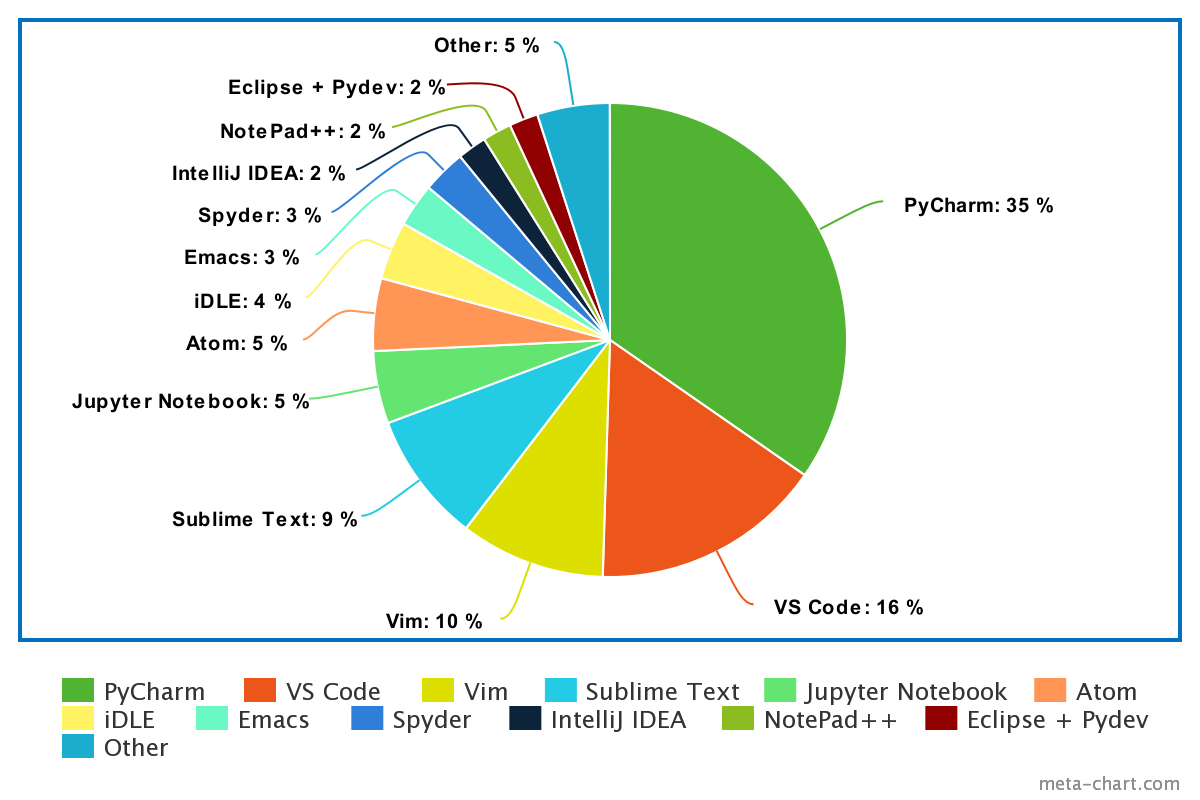
\includegraphics[scale=0.25]{pie.png}
\end{center}
\caption{Populari Editori i IDE za rad sa Python-om}
\label{fig:pie}
\end{figure}

Moguće je debagovati korišćenjem nekih editora koji podržavaju jezik Python. Na prethodnoj slici \ref{fig:pie} možemo videti neke od njih.

\section{Debagovanje u okružnju PyCharm}
U ovom delu pokazaćemo kako debagovati u razvojnom okruženju PyCharm. Da bi započeli debagovanje prvo moramo postaviti \emph{tačke prekida (eng. breakpoint)} koji će signalizirati debageru  da treba da se zaustavi na određenom mestu u k\^{o}du i da nam da izveštaj stanja u tom trenutku. Breakpoint postavljamo tako što klinemo na prazninu uz levu marginu.

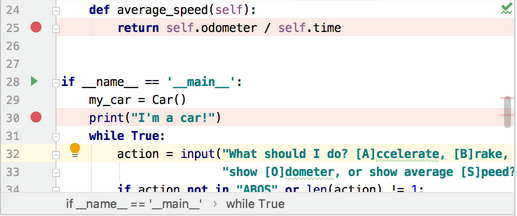
\includegraphics[scale = 0.4]{1}

Znaćemo da je Breakpoint uspešno postavljen pojavom crvenog kružića\cite{pyCharm}. Prilikom pokretanja main funkcije našeg programa možemo izabrati opciju Debug, ovo će otvoriti \emph{Debug tool window} u kome možemo pokrenuti naš python k\^{o}d I gde ćemo dobijati sve informacije o izvršavanju. Informacije koje dobijamo mogu sadržati poruke o greškama, ne uhvaćene izuzetke, vrednosti promenljivih (u svom zasebnom prozoru) i druge\cite{pyCharm}. PyCharm se automatski zaustavlja ukoliko naiđe na izuzetak koji nije uhvaćen inače se zaustavlja na lokaciji prvog breakpoint-a\cite{pyCharm}. Ukoliko program ima više niti dobićemo posebne prozore za svaku od njih\cite{pyCharm}.
\subsection{Detaljno debagovanje}
Šta ako želimo da posmatramo izvršavanje našeg k\^{o}da korak po korak? Da li ovo znači da moramo postaviti breakpoint u svakoj liniji? Odgovor je ne, PyCharm debugger poseduje, u svom Debug tool window, takozvani \emph{Stepping toolbar}.

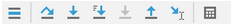
\includegraphics[scale = 0.6]{2}

Često korišćene opcije koje su nam na raspolaganju su:
\begin{itemize}
\item  Step Over
\item  Step Into
\item Step Into My Code
\end{itemize}
Step Over jednostavno prelazi na sledeću liniju koda (linija na kojoj se trenutno nalazimo biće osenčena u editoru). Step Into opcija će nas voditi kroz biblioteke i funkcije koje koristimo kada na njih naiđemo\cite{pyCharm}.
\begin{lstlisting}[language = Python, caption={Primer neki}]
 x = random.nextInt();
 y = f(x);
\end{lstlisting} 
 ovaj kod će nas odvesti u biblioteku Random ako na ovoj liniji koristimo opciju Step Into odnosno u definiciju funkcije f, ovo često ne želimo pa koristimo opciju Step Into My Code koja će nas zadržati u našem k\^{o}du\cite{pyCharm}. 
\subsection{Posmatranja (Watches)}
PyCharm nam omogućava da posmatramo promenljive kroz izvršavanje našeg programa. U tabu debagera \emph{Variables} se nalaze sve promenljive koje postoje i koje su vidljive u trenutnom stanju izvrsavanja i na trenutnoj lokaciji u kodu kao i njihov tip i vrednost\cite{pyCharm}. Ako klinknemo na \emph {plus} u gornjem levom uglu dobijamo opciju da dodamo bilo koju promenljivu i ona će biti praćena uvek bez obzira na to gde se ona nalazi, da li je trenutno vidljiva i da li je uopšte definisana\cite{pyCharm}.
\subsection{Inline Debugger}
Jedna od opcija koju nam pruža PyCharm jeste da klikom na Break point odmah dobijamo informacije o našim promenljivima i objektima odmah u editoru u vidu komentara. Ova opcija je podrazumevana i može se promeniti u Debug Tool window-u\cite{pyCharm}.


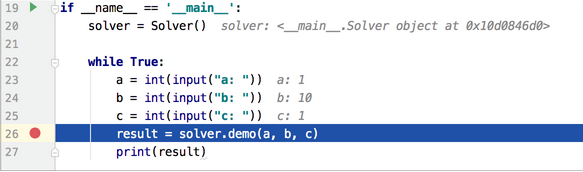
\includegraphics[scale = 0.4]{3}
\subsection{Evaluacija izraza}
Poslednja opcija koja se nalazi na Stepping Toolbar-u je opcija za evaluaciju izraza. Ovo opcija nam omogućava da izračunamo vrednost neke promenljive koja nam je trenutno u opsegu ili nekog izraza\cite{pyCharm}. Pitanje koje se postavlja je zašto bi ovo koristili jer isto možemo dobiti korišćenjem Posmatranja. Ovo je tačno ali evaluacijom možemo uraditi nešto što Posmatranje ne može, a to je da postavimo vrednost nekoj promenljivoj\cite{pyCharm}. Ovo je jako korisno jer mozemo testirati naš kod za neke kritične vrednosti tako što ćemo na `vestacki` nacin da dodeljujemo vrednosti promenljivima koje će nas dovesti do tog kriticnog stanja.

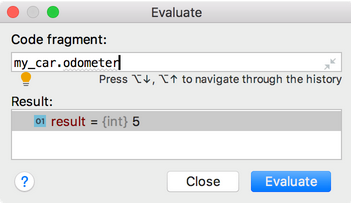
\includegraphics[scale = 0.4]{4}
\section{Zaključak}
\label{sec:zakljucak}

Pajton je široko rasprostranjen i popularan jezik zbog svoje jednostavnosti, lakoće u pisanju i pristupačnosti za početnike. Ne odlikuje ga stroga tipiziranost i sam jezik omogućava pisanje na višem, apstraktnijem nivou. To nekada znači da nam on više “prašta” nego što bi trebalo i da se mogu “potkriti” razne greške. Zato je neophodno imati dobre alate za debagovanje koji mogu delovati kao ključni posrednici u pisanju korektnog koda, čineći taj proces efikasnim i nenapornim. Tako imamo odličnu kombinaciju udobnosti u pisanju i pouzdanosti koda. Od preventivnih mera kao što je hvatanje izuzetaka i jednostavnijih metoda debagovanja kao što su interakcija sa programom preko terminala i korišćenje print naredbi, zatim formalne naučne metode, pa sve do složenijih biblioteka logging, pdb i okruženja PyCharm, čitaocu je sada poznato više mehanizama debagovanja, koji predstavljaju samo jedan deo širokog opusa mogućnosti. Postoji mnogo više alata i oni sa pomenutim dele ključne koncepte. Za većinu njih postoji opsežna dokumentacija i dosta pomoći na internetu, što zbog popularnosti alata, što zbog popularnosti samog jezika. Ostavlja se čitaocu da preko datih objašnjenja izabere odgovarajući metod na osnovu svojih potreba i preferensi.


\addcontentsline{toc}{section}{Literatura}
\appendix
\bibliography{seminarski} 
\bibliographystyle{plain}

\newpage

\appendix
\section{Dodatak}
Ovde pišem dodatne stvari, ukoliko za time ima potrebe.


\end{document}
